
%-----------------------------------------------------------------------
%   Introduction
%-----------------------------------------------------------------------
\section{Introduction}
\emph{Since the discovery of the Standard Model (SM) Higgs boson at the CERN
LHC experiments and subsequent measurement of its
parameters, all fundamental parameters of the SM have been measured
directly and with remarkable precision.
To further establish the validity of the theory of electroweak
interactions, validate the mechanism of electroweak symmetry breaking
and the mechanism of the generation of particle masses, further
high-precision electroweak measurements have to be performed.
Such high-precision measurements are also often considered as a portal
to new physics, since non-SM contributions, as for instance
loop-insertions, may yield significant deviations for some precisely
measurable and calculable observables.
The greatly enlarged kinematic reach to higher scales in comparison to
HERA and the large targeted luminosity will allow for the first time
high-precision electroweak measurements in $ep$.}

\emph{The LHeC experimental conditions offer the opportunity for unique measurements of electroweak
parameters, which are often complementary to other experiments, such
as proton-proton or electron-positron collider experiments or low
energy neutrino or muon scattering experiments.
Among many other quantities, unique measurements of the weak couplings
of the light quarks, $u$ and $d$, can be performed due to the
important contributions of valence quarks in the initial state, as well as scale
dependent measurements of weak interactions, since deep-inelastic $ep$
scattering is mediated through space-like momentum transfer
($t$-channel exchange).}

%
In this article we study the sensitivity of inclusive NC and CC cross
section at LHeC to electroweak parameters.


\paragraph{H1 paper intro with references}
\emph{Since the discovery of weak neutral currents in 1973~\cite{Hasert:1973ff,Haidt:2015bgg},
the Glashow-Weinberg-Salam
model~\cite{Glashow:1961tr,Weinberg:1967tq,Weinberg:1971fb,Weinberg:1972tu,Salam:1964ry,Higgs:1964ia,Higgs:1964pj,Englert:1964et}
has been established as the theory of electroweak (EW) interactions and as
the core of the Standard Model (SM) of particle physics.
Already since these early times, deep-inelastic lepton-hadron
scattering (DIS) experiments with longitudinally polarised electron beams have provided indispensable
results~\cite{Prescott:1978tm,Prescott:1979dh} for its great
success.
%                                                                                                                       
Nowadays, EW theory has been tested in great detail at
lower scales with muon life-time measurements~\cite{Tishchenko:2012ie}
and neutrino scattering experiments~\cite{Fogli:1988tv,Blondel:1989ev,Allaby:1987vr,McFarland:1997wx,Zeller:2001hh},
with precision measurements at the $Z$ pole and at even higher
scales~\cite{ALEPH:2005ab,Chatrchyan:2011ya,Schael:2013ita,Aaij:2015lka,Aad:2015uau,Aaltonen:2018dxj}.
%                                                                                                                       
The H1 Collaboration has performed first studies of weak interactions at
the HERA electron-proton collider in 1993.
The measurement of the total charged-current cross section
demonstrated for the first
time the presence of the $W$-boson propagator~\cite{Ahmed:1994fa}.}



%-----------------------------------------------------------------------
%   Theory
%-----------------------------------------------------------------------
\clearpage
\section{Electroweak effects in inclusive NC and CC DIS cross sections}
\label{sec:theo}
%
Inclusive NC DIS cross sections are expressed in terms of
generalised structure functions $\tilde{F}_2^\pm$, $x\tilde{F}_3^\pm$
and $\tilde{F}_{\rm L}^\pm$ at EW leading order (LO)
as
\begin{equation}
  \frac{d^2\sigma^{\rm NC}(e^\pm p)}{dxd\Qsq} = \frac{2\pi\alpha^2}{xQ^4}\left[Y_+\tilde{F}_2^\pm(x,\Qsq) \mp Y_{-}  x\tilde{F}_3^\pm(x,\Qsq) - y^2 \tilde{F}_{\rm L}^\pm(x,\Qsq)\right]~,
  \label{eq:cs}
\end{equation}
where $\alpha$ denotes the fine structure constant and $x$ the
Bjorken scaling variable.
The terms $Y_\pm = 1\pm(1-y)^2$ contain the helicity dependence of
the process, where $y$ denotes the inelasticity of the process.
The  generalised structure functions are then separated into contributions
from pure $\gamma$- and $Z$-exchange and their interference~\cite{Klein:1983vs}:
\begin{align}
  \tilde{F}_2^\pm
  &= F_2
  -(\ve\pm P_e\gae)\varkappa_ZF_2^{\gamma Z}
  +\left[(\ve\ve+\gae\gae)\pm2P_e\ve\gae\right]\varkappa_Z^2F_2^Z~,
  \\
  \tilde{F}_3^\pm
  &=~~
  -(\gae\pm P_e\ve)\varkappa_ZF_3^{\gamma Z}
  +\left[2\ve\gae\pm P_e(\ve\ve+\gae\gae)\right]\varkappa_Z^2F_3^Z~.
  \label{eq:strfun}
\end{align}
Similar expressions hold for $\tilde{F}_L$.
%
In the naive quark-parton model, which corresponds to the LO QCD
approximation, the structure functions are calculated as
\begin{align}
  \left[F_2,F_2^{\gamma Z},F_2^Z\right]
  &= x\sum_q\left[Q_q^2,2Q_q\vq,\vq\vq+\aq\aq \right]\{q+\bar{q}\}~,
  \label{eq:last1}
  \\
  x\left[F_3^{\gamma Z},F_3^Z\right]
  &= x\sum_q\left[2Q_q\aq,2\vq\aq\right]\{q-\bar{q}\}~,
  \label{eq:last2}
\end{align}
and it is easily recognized that those are closely related
to the quark and anti-quark momentum distributions, $xq$ and $x\bar{q}$.
In eqs.~\eqref{eq:strfun} and~\eqref{eq:gV-LO}, the variables $g_V^{e/q}$
and $g_A^{e/q}$ stand for the vector and axial-vector couplings of the
lepton or quarks to the $Z$ boson, and the coefficient $\varkappa_Z$
accounts for the $Z$-boson propagator and the normalisation of the  weak contributions.
%
Both parameters are given by electroweak theory.
The (effective) coupling parameters
depend on the electric charge, $Q_{q/e}$, in units of the positron charge,
and on the third component of the weak-isospin of the fermion, $I^3_{{\rm L},q/e}$.
Using $\sw=1-\tfrac{M_W^2}{M_Z^2}$, they are given by
\begin{align}
  g_A^{f} &= \sqrt{\rho_{\text{NC}, f}} I^3_{{\rm L},f}
  \label{eq:gA-LO} \,, \\
  g_V^{f} &= \sqrt{\rho_{\text{NC}, f}} \left(I^3_{{\rm L},f} - 2
  Q_{f} \kappa_{\text{NC}, f}\ \sw \right)
  \label{eq:gV-LO} \,.
\end{align}
The form factors $\rho_{\text{NC}, f}$ and $\kappa_{\text{NC}, f}$
represent the universal higher-order corrections, and due to their
\Qsq\ dependence the couplings become `effective'.
%The latter has been measured with highest precision
%in muon-decay experiments~\cite{Tishchenko:2012ie}.
%
The coefficient $\varkappa_Z$ is calculated as
\begin{equation}
  \varkappa_Z(\Qsq)
  = \frac{\Qsq}{\Qsq+M^2_Z}
  \frac{1}{4\sw \cos^2\theta_W}
  = \frac{\Qsq}{\Qsq+M^2_Z}
  \frac{\gf M_Z^2}{2\sqrt{2}\pi\alpha}~,
\end{equation}
%i.e.\ taking into account either the weak mixing angle, $\sw=1-\mW^2 /
i.e.\ taking into account $\sw$, or alternatively using the Fermi coupling constant $\gf$.

In order to perform predictions in LO electroweak theory only two independent
parameters are needed in addition to $\alpha$.
At higher orders, loop corrections involve a non-negligible dependence
on further parameters, where the most important ones are $M_t$
and $M_H$ and hadronic contributions.


In the LO approximation, the CC DIS cross section is written as
\begin{equation}
  \frac{d^2\sigma^{\rm CC}(e^\pm p)}{dxd\Qsq}
  = \left(1 \pm P_e\right)
  \frac{\gf^2}{4\pi x}
  \left[\frac{m_W^2}{m_W^2+\Qsq}\right]^2
  \left(Y_+ W_2^\pm(x,\Qsq) \mp Y_{-} xW_3^\pm(x,\Qsq)
  - y^2 W_{\rm L}^\pm(x,\Qsq)\right)~.
  \label{eq:cc-cs}
\end{equation}
In the simplified quark-parton model the structure
functions $W_2^\pm$ and $xW_3^\pm$ are obtained from the parton
distribution functions, while $W_{\rm L}^\pm = 0$:
An incoming electron can scatter only with
positively charged quarks,
\begin{equation}
  W_2^- =
  x \left( U + \overline{D} \right)
  \, ,
  \quad xW_3^- =
  x \left( U - \overline{D} \right)
  \, ,
  \label{eq:w23el-LO}
\end{equation}
while positrons scatter only with negatively charged quarks,
\begin{equation}
  W_2^+ =
  x \left( \overline{U} + D \right)
  \, {~~\text{and}~~}
  \quad xW_3^+ =
  x \left( D - \overline{U} \right)
  \, ,
  \label{eq:w23po-LO}
\end{equation}
using the parton combinations
$U = u+c$, $\overline{U} = \bar{u} + \bar{c}$, $D = d+s$
and $\overline{D} = \bar{d} + \bar{s}$.
{\color{green} Introduce \Qsq dependent form factors.}

Due to renormalisation of the corrections and the choice of
input parameters the calculations become scheme dependent.
In this study we adopt the on-shell scheme using \mz\ and \mw\ as input
parameters to the calculations.

\paragraph{References}
In the on-shell (OS) scheme~\cite{Sirlin:1980nh,Sirlin:1983ys},

higher-order corrections enter through the
quantity $\dr = \dr(\alpha, m_W, m_Z, m_H, m_t, \ldots)$
\cite{Sirlin:1980nh}, which describes corrections to the muon
decay beyond the tree-level~\cite{Bohm:1986rj,Hollik:1988ii}.

\emph{One-loop EW corrections have been calculated
in refs.~\cite{Bohm:1986na,Bardin:1988by,Hollik:1992bz}
for NC and in refs.~\cite{Bohm:1987cg,Bardin:1989vz} for CC
scattering (see also ref.~\cite{Heinemann:1998kk} for a study of
numerical results).}

\gf\ measurement~\cite{Tishchenko:2012ie}



% -------------------------------------------------------------------
%
% -------------------------------------------------------------------
\clearpage
\section{The inclusive DIS cross section and LHeC}
The contributions of electroweak effects to the inclusive NC and CC
DIS cross sections can well be illustrated for
the single-differential cross sections for polarised $e^-p$ scattering
as function of \Qsq.
These are diplayed in figure~\ref{fig:dSigma}
for LHeC electron beam energies of $E_e=50\,\GeV$ and 60\,\GeV, and a
proton beam energy of $E_p=7000\,\GeV$.
The LHeC predictions are compared to measurements at HERA
($E_e=27.6\,\GeV$ and $E_p=920\,\GeV$, with $P_e=0$) and their
predictions. 
%
\begin{figure}[htb]
  \centering
  \includegraphics[width=0.52\textwidth]{plot_GraphsDsigmaDQ2_LHeC}
  \caption{{Single differential inclusive DIS cross sections for
      polarised $e^-p$ NC 
      and CC DIS at the LHeC for two different electron beam energies
      ($E_e=50\,\GeV$ and 60\,\GeV). Cross sections for longitudinal
      electron beam
      polarisations of $P_e=-0.8$ and $+0.8$ are displayed.
      For comparison also measurements at center-of-mass energies
      of $\sqrt{s}=920$ by H1 at HERA for unpolarised ($P=0\,\%$)
      electron beams are displayed.
  }}
  \label{fig:dSigma}
\end{figure}


%
At lower values of \Qsq, the NC cross sections are dominated by
photon-exchange contributions, represented by 
the structure function $F_2$ (c.f.~eq.\,\eqref{eq:strfun}), while the CC
cross section are suppressed with respect to the NC ones and are
almost independent on \Qsq.
This is due to the mass of the $W$ boson, since
$\Qsq\ll\mW^2$ and thus the propagator term becomes
$\tfrac{\mW^2}{\mW^2+\Qsq} \simeq 1$.
At \Qsq\ values around the electroweak scale, $\Qsq\approx\mZ^2$,
weak contributions to the NC cross sections become important.
For instance, this can be observed as the NC cross section becomes
dependent on the longitudinal beam polarisation, $P_e$, and the cross
sections for positive and negative polarisations start to differ
significantly.
For CC, the impact of the longitudinal beam polarisation is of course
much more prominent, since CC is mediated exclusively by weak
interactions and the cross section scales linearly with the
size of $P_e$ (c.f.~Eq.\,\eqref{eq:cc-cs}).
Note, since DIS is mediated in the space-like regime, no resonance of
a weak boson is present in the \Qsq dependent cross section.
%Also for NC cross sections the 
%polarisation effects are significant in kinematic regions, where
%$\gamma Z$ and pure $Z$  exchange are important.
With a reduced electron beam energy of $E_e=50\,\GeV$, the
center-of-mass energy reduces to $1.18\,\TeV$ and
in the exemplary range from $10\,000<\Qsq<100\,000\,\GeVsq$
the reduced NC or CC cross sections are lower by about 10 to 15\,\%.
At even higher \Qsq\ values the difference between $E_e=50\,\GeV$ or
60\,\GeV cross sections further increases.
%and also the
%sensitivity to electroweak parameters in NC exchange reduces
%accordingly.
%





% -------------------------------------------------------------------
%
% -------------------------------------------------------------------
\clearpage
\section{LHeC pseudo data}
\label{sec:data}
In this section, the details of the LHeC pseudo data\,\footnote{In the
following, the simulated \emph{pseudo data} is simply denoted as
`data' in order to facilitate reading.}
as used for the upcoming extraction of electroweak parameters are discussed.

In this analysis a recent simulation of double-differential inclusive
NC and CC DIS cross section data as function of \Qsq\ and Bjorken-$x$
are exploited. 
The data sets include electron and positron data, different lepton
beam polarisation states, and different proton beam energies.
Since the actual layout of the LHeC energy-recovery linac for the lepton
beam is not yet decided, we will study scenarios for two lepton beam
energies of either $E_e=50\,\GeV$ or 60\,\GeV in the following,
whereas the nominal LHC proton beam energy of $E_p=7000\,\GeV$ is
considered.
In addition, a small sample with reduced  $E_p$ of only 1000\,GeV is
further simulated.
For each beam setup NC and CC DIS data are simulated and
a summary of the data sets is given in Table~\ref{tab:datasets}.
\begin{table}[bht]
  \centering
  \small
  \begin{tabular}{lccccccc}
    \toprule
    Data set & Processes & $E_p$ [TeV] & $Q_e$ & $P_e$ &
    $\mathcal{L}$ [fb$^{-1}$] & \Qsq\ range [\GeVsq] & No. of data points (NC,CC)\\
    \midrule
    D1 & NC,CC &  7  & $-1$ &  $-0.8$ & 1000 & 5 -- $10^6$ & 100 \\ % D4
    D2 & NC,CC &  7  & $-1$ &  $+0.8$ & 10   & 5 -- 1\,000\,000 & 100 \\ % D8
    D3 & NC,CC &  7  & $+1$ &  $ 0  $ & 10   & 5 -- 1\,000\,000 & 100 \\ % D7
    D4 & NC,CC &  1  & $-1$ &  $ 0  $ & 1    & 5 -- 1\,000\,000 & 100 \\ % D5
    \bottomrule
 \end{tabular}
  \caption{Summary of simulated data sets used.
    Each data set is simulated for the two studied
    electron beam energies of $E_e=50\,\GeV$ and 60\,\GeV.
    {\color{red}last twp columns!}
    {\color{blue}to be checked, if Ee=50 and 60 used these settings.}
  }
  \label{tab:datasets}
\end{table}
The vast majority of the data will be collected with an electron
($Q_e=-1$) beam and with a beam longitudinal polarisation
of $P_e=-0.8$, reaching an integrated luminosity of about
$\mathcal{L}\simeq1000\,\textrm{fb}^{-1}$.
This will allow measurements of NC and CC DIS cross sections up to values of
$\Qsq\simeq1\,000\,000\,\GeVsq$.
A considerably smaller data sample will be collected with a positive
electron beam polarisation of $P_e=+0.8$. For this sample, an
integrated luminosity of 10\,fb$^{-1}$ is assumed.
Another data sample will be collected with a positron beam, where
an unpolarised beam is assumed.
The technical limitations for the generation of positrons put
constraints on the achievable beam current and thus on the instaneous
luminosity. Therefore, an
integrated luminosity of (only) 10\,fb$^{-1}$ is assumed for this sample.
Nonetheless, this will allow measurements with positrons up to
\Qsq\ values of 500\,000\,\GeVsq.
Yet another data sample will be collected with a reduced proton beam
energy, which will mainly be used for measurements of $F_L$ and access
higher values of $x$.
For this sample an integrated luminosity of 1\,fb$^{-1}$ is assumed.
All data is restricted to $\Qsq\geq5\,\GeVsq$ in order to avoid
regions, where higher order QCD effects are important, and may
deteriorate PDF determinations, while the
low-\Qsq region has anyhow only very low sensitivity to EW parameters.
CC DIS data are simulated for $\Qsq\geq100\,\GeVsq$, and lower \Qsq
values may not be measurable due to trigger limitations.

The simulated data points account for the acceptance of the LHeC
detector, the kinematic reconstruction, and trigger restrictions.
The latter, for instance, restricts CC DIS measurements to
$\Qsq\gtrsim100\,\GeVsq$.
The resulting kinematic plane of the simulated data points is displayed, for
instance, in Ref.~\cite{AbdulKhalek:2019mps} (where, however, slightly
different assumptions on the data uncertainties have been used).

The data include a full set of systematic uncertainties and
the individual sources are summarised in Table~\ref{tab:uncert}.
\begin{table}[bht]
  \centering
  \small
  \begin{tabular}{lc}
    \toprule
    Source of uncertainty & Uncertainty \\
    \midrule
    Scattered electron energy scale $\Delta E_e' /E_e'$ & 0.1 \% \\
    Scattered electron polar angle  & 0.1\,mrad \\
    Hadronic energy scale $\Delta E_h /E_h$ & 0.5\,\% \\
    %calorimeter noise (only $y < 0.01$) & 1-3\,\% \\
    Radiative corrections & 0.3\,\% \\
    Photoproduction background ($y > 0.5$) & 1\,\% \\
    Uncorrelated uncertainty & 0.5\,\% \\ % Global efficiency error
    Luminosity uncertainty & 1.0\,\% \\
    \bottomrule
 \end{tabular}
\caption{
  Assumptions on the size of uncertainties from various sources used
  in the simulation of the NC cross sections.
  The top three are uncertainties on the calibrations and are
  propagated to the cross sections.
  %which are transported to
  %provide correlated systematic cross section errors.
  The lower four are uncertainties by various sources and directly
  assigned to the cross section.
}
\label{tab:uncert}
\end{table}
For the bulk of the phase space, the `electron' reconstruction method
is employed and important uncertainties originate from the scattered
electron energy scale and its polar angle measurement, where
uncertainties of $\Delta E_e' /E_e'=0.1\,\%$ and
$\Delta\theta^\prime_e=0.1$\,mrad are assumed, respectively.
However, at lower values of $y$ the so-called `mixed' reconstruction
method~\cite{Blumlein:1990dj} is employed, which makes use of the
measurement of the hadronic final state for $y$, and $x=\Qsq/(sy)$. %$y_h=\tfrac{\Sigma}{2E_e}$.
For the measurement of the hadronic final state,
an uncertainty on the hadronic energy scale $\Delta E_h/E_h=0.5\,\%$
is imposed.
Furthermore, uncertainties on the QED radiative corrections of
0.3\,\%, and uncertainty on the background from photoproduction events
of $1.0\,\%$ at the high-$y$ region is assumed.
The statistical uncertainty is taken to be at least 0.1\,\%.
A global normalisation uncertainty, including the luminosity
uncertainty, of 1\,\% is considered. 

A number of further potential uncertainty sources is
summarised in an uncorrelated uncertainty component of 0.5\,\%.

These data samples have been simulated mainly for the purpose of performing
reliable studies for PDF determinations, which are mainly sensitive to
the lower \Qsq region.
In contrast, the present study on electroweak parameters is mainly
sensitive to the high \Qsq region.
For technical reasons, and for simplicity, an \emph{ad-hoc} $x$-\Qsq
grid for the simulated data points was chosen.
Though, the upcoming real data may allow a much finer binning, in
particular at medium $x$ values or at higher \Qsq.
With the given treatement of fully correlated, or fully uncorrelated
uncertainty sources, a finer binning can
be simulated  to a very good approximation  by changing the size of
the uncorrelated uncertainty. 
In the following, an alternative scenario is considered, where we assume
a two times finer bin-grid in $x$, as well as in \Qsq.
\emph{This is simply emulated by using an uncorrelated uncertainty of $0.25\,\%$.
{\color{green} We keep a minimum statistical uncertainty on every data
  point of 0.1\,\%.}}

%\footnote{Due to performance
%  reasons, the pseudo-data are generated for a rather coarse bin grid. With a
%  binning, which is closely related to the resolution of the LHeC
%  detector, a much finer binning in $x$ and \Qsq are feasible. Already
%  such a change would alter the uncertainties of the fit parameters.
%  However, such an effect can be reflected by a
%  changed uncorrelated uncertainty, and a value of 0.25\,\% appears
%  like an optimistic, but achievable,  alternative scenario. },

In summary, we study four sets of data samples, as summarised in Table\,\ref{tab:scenarios}.
\begin{table}[hbt]
  \centering
  \small
  \begin{tabular}{lccc}
    \toprule
    Scenario name & $E_e$ & Bin grid  & $\delta_\textrm{unc}$\\
    \midrule
    LHeC-50a  &   50\,\GeV&  nominal             &  0.5\,\%  \\
    LHeC-50b  &   50\,\GeV&  4$\times$ nominal   &  0.25\,\% \\
    LHeC-60a  &   60\,\GeV&  nominal             &  0.5\,\%  \\
    LHeC-60b  &   60\,\GeV&  4$\times$ nominal   &  0.25\,\% \\
    \bottomrule
 \end{tabular}
  \caption{
    Summary of the naming convention of the LHeC scenarios studied.
    The last column indicates the technical realisation in the data
    tables of the chosen bin grid.
  }
  \label{tab:scenarios}
\end{table}







%-----------------------------------------------------------------------
%   Methodology
%-----------------------------------------------------------------------
\clearpage
\section{Methodology of a combined EW and QCD fit}
The expected uncertainties of the electroweak parameters of interest are
determined in a combined fit together
with the PDFs to the inclusive NC/CC DIS data (denoted in the
following as `PDF+EW' fit).
The full set of statistical and systematic uncertainties of the data
are considered. 
In this fit, also parameters of the PDFs are determined, since at the
time of the LHeC, PDFs will predominantly be determined from these
inclusive NC/CC DIS data under consideration.
In order to account for the correlation between PDF uncertainties,
which mainly represent the propagated uncertainties of these 
LHeC inclusive DIS data, and the EW parameter under consideration, the
PDFs have to be determined simultaneously in this fit.
In doing so, this provides the inherent sensitivity of the LHeC data
to EW parameters.


In the calculation NNLO pQCD calculations with the zero-mass variable
flavor number scheme are used, as implemented in
QCDNUM~\cite{Botje:2010ay,Botje:2016wbq}.  
For the PDF evolution or the structure function calculations, no QED
or EW
contributions~\cite{DeRujula:1979grv,Kripfganz:1988bd,Blumlein:1989gk}
are included.
These are expected to be negligible~\cite{Spiesberger:1994dm},
in particular since these 
contributions will not add additional sensitivity 
to the EW parameters of interest, and as such will not change the
expected uncertainties in the present study.
The $x$ dependent PDFs are parameterised at a scale of
$\mu_0=1.3784\,\GeV$, i.e.\ below the charm mass.
Five orthogonal PDF linear combinations are chosen to be parameterised
at $\mu_0$: the $u$ and
$d$ valence quark distributions ($xu$,$xv$), the $u$-type and $d$-type
anti-quark distributions ($x\bar{U}$,$x\bar{D}$), and the gluon
distribution ($xg$).
The chosen parameterisation follows closely previous LHeC PDF
studies~\cite{AbelleiraFernandez:2012cc,Klein:1564929}, 
which are closely related to HERAPDF-style
PDFs~\cite{Adloff:2000qk,Abramowicz:2015mha,Andreev:2017vxu}. 
The following functional form is chosen
\begin{equation}
  xf = f_A x^{f_B} (1-x)^{f_C} (1+f_Dx+f_Ex^2) -
      f_{A^\prime}x^{f_{B^\prime}}(1-x)^{0.25}\,,
\end{equation}
where $f$ denotes any of the five linear combinations.
The second summand is considered only for the gluon distribution\footnote{
Although, the second term is commonly considered to be of importance for PDF
determinations as it introduces
additional freedom at lower values of $x$ and since the
LHeC probes $x$ regions as low as $5\cdot10^{-6}$, it is found to has
no significant impact on the resulting uncertainties of the
electroweak parameters.}.
The normalisation parameters are determined through the quark number
sum-rule ($u_A$, $d_A$) or the momentum sum-rules ($A_g$), or are calculated
as $\bar{U}_A=\bar{D}_A(1-0.4)$.
Furthermore, we use $\bar{D}_B=\bar{U}_B$.
Finally, altogether 13 parameters  of the PDFs are determined in each
of the fits
($g_B$, $g_C$, $g_{A^\prime}$, $g_{B^\prime}$, $u_B$, $u_C$, $u_E$,
$d_B$, $d_C$, $\bar{U}_C$, $\bar{D}_A$, $\bar{D}_B$, $\bar{D}_C$), while
all other parameters are set to zero.
The actual values of the PDF parameters are not of noteworthy
relevance here, and are set to values, as they can be obtained from a
fit to HERA data~\cite{Aaron:2012qi,Andreev:2017vxu}. 

EW effects are included into the calculation by considering the full
set of 1-loop electroweak corrections (see sect.~\ref{sec:theo})
and are implemented in the
programm EPRC~\cite{Spiesberger:1995pr}.
{\color{red} more to add here...}

The $\chi^2$ quantity which is subject to the minimisation and
error propagation is based on normal-distributed relative
uncertainties,
\begin{equation}
  \chi^2 =\sum_{ij} \log{\frac{\varsigma_i}{\sigma_i}}V^{-1}_{ij}\log{\frac{\varsigma_j}{\sigma_j}}
\end{equation}
where the sum runs over all data points $\varsigma_i$ and their
corresponding predictions, $\sigma_i$.
The covariance matrix $V$ represents the relative uncertainties of the
data points.
The Minuit library is employed and the resulting uncertainties of the fit
parameters are calculated using the HESSE or MINOS algorithm~\cite{James:1975dr}.
For our study, we set the data values equivalent to the predictions,
i.e.\ our data represent an \emph{Asimov data set}~\cite{Cowan:2010js}.
It it is noteworthy, that with the chosen $\chi^2$ definition, the actual
size of the cross section at a given point does not enter the
calculation of the uncertainties, but only the relative size of the
uncertainties are of relevance.






%-----------------------------------------------------------------------
%   Results: mass parameters
%-----------------------------------------------------------------------
\clearpage
\section{Mass determinations of the weak bosons}
\label{sec:mass}
In this section, first, a determination of the $W$-boson mass, \mW,
then the $Z$-boson mass, \mZ, then a combined determination of \mW\ and
\mZ, and finally a possible determination of the Higgs-boson mass,
\mH, is discussed. 
The expected uncertainties for a determination of the weak boson
masses are determined in the PDF+EW fit, where one of the masses is
determined together with the PDFs.
The other mass parameters are taken as external input in this
fit.
All parameters are defined in the on-shell scheme.


For a determination of the $W$-boson mass, expected uncertainties of
\begin{alignat}{2}
  \Delta\mW(\text{LHeC-60a})&=\pm5_{({\rm exp})}\pm8_{({\rm PDF})}\,\MeV  =\,&& 10_{\text{(tot)}}\,\MeV{\rm ~~and~~} \\
  \Delta\mW(\text{LHeC-50a})&=\pm8_{({\rm exp})}\pm9_{({\rm PDF})}\,\MeV  =\,&& 12_{\text{(tot)}}\,\MeV
\nonumber
\end{alignat}
are found for the scenarios LHeC-60a and LHeC-50a (c.f.\
section\,\ref{sec:data}), and uncertainties of
\begin{alignat}{2}
  \Delta\mW(\text{LHeC-60b})&=\pm3_{({\rm exp})}\pm5_{({\rm PDF})}\,\MeV =\,&& 6_{\text{(tot)}}\,\MeV{\rm ~~and~~} \\
  \Delta\mW(\text{LHeC-50b})&=\pm6_{({\rm exp})}\pm6_{({\rm PDF})}\,\MeV =\,&& 8_{\text{(tot)}}\,\MeV
\nonumber
\end{alignat}
are obtained for LHeC-60b and LHeC-50b, respectively.
%
An artificial breakdown into experimental and PDF uncertainties is
obtained by repeating the fit with PDF parameters kept fixed, which
yields the \emph{exp} uncertainty, while the PDF uncertainty is then
calculated as the quadratic difference from the total uncertainty.
The size of the uncertainty component associated to the PDFs is found
to be  of similar size as the \emph{exp} uncertainty.
%
The expected total uncertainties are displayed in
figure~\ref{fig:mW} (left) and compared to the values obtained by
LEP2~\cite{Schael:2013ita}, Tevatron~\cite{Group:2012gb},
ATLAS~\cite{Aaboud:2017svj} and the PDG value~\cite{Tanabashi:2018oca,PDG19}.
%
It is found, that the LHeC measurement will yield the smallest
experimental uncertainties in a single experiment\,\footnote{In
  figure~\ref{fig:mW}, the values from LEP2 and Tevatron represent
  combined results taking into account measurements from independent
  experiments and thus benefit from a reduction of the systematic
  uncertainties in the combination procedure. Similarly, the
  PDG world average value.}.
The LHeC measurement will further be even superior than the current
world average. 
As such, a detailed assessement of associated theoretical
uncertainties will be needed, where the largest source is due to the
top-quark mass due its contribution to \dr. An uncertainty of the
top-quark mass of $0.5\,\GeV$ will yield an additional uncertainty of
$\Delta\mW=2.5\,\MeV$. 


The full dependence of the expected total experimental uncertainty
$\Delta\mW$ on the size of the uncorrelated uncertainty component
%and the normalisation uncertainty
is displayed in figure~\ref{fig:mW} (right).
\begin{figure}[thbp]
    \centering
    \includegraphics[width=0.42\textwidth]{alphas_summary_W-bosonMass}
    \hskip0.05\textwidth
    \includegraphics[width=0.42\textwidth]{mW_uncorr}
    \caption{
      Left: Measurements of the $W$-boson mass  at fixed top-quark
      and $Z$-boson masses at LHeC for different LHeC
      scenarios in comparison with todays
      measurements~\cite{Group:2012gb,Schael:2013ita,Aaboud:2017svj}
      and the  world average value (PDG19)~\cite{Tanabashi:2018,PDG19}.
      For LHeC, prospects for $E_e=60\,\GeV$ and 50\,\GeV are
      displayed for the two scenarios `a' and `b' (see text).
      Right: Comparison of the precision for $M_W$ for different assumptions of the uncorrelated
      uncertainty of the pseudo-data.
      The uncertainty of the world average value is displayed as horizontal line.
      The scenarios `a' and `b' are indicated by the vertical line.
    }
    \label{fig:mW}
\end{figure}
Note, for the scenarios LHeC-60a and LHeC-50a an uncorrelated
uncertainty of 0.5\,\% is used, and for the `b'-scenarios a size of 0.25\,\%.
It is well visible, that a good control of the uncorrelated
uncertainty component, or respectively a higher resolution that yields
a potentially finer bin grid, considerably improves the uncertainties
of the $W$-boson mass measurement.
%


{\color{blue}Conclusion?)
\color{red}
  The measurement of \mW\ in DIS constitutes an highly important
  alternative determination of \mW, ... $t$-channel vs.\ $s$-channel,
  DIS vs.\ $ee$ and $pp$. $W$ mass not produced on-shell, but a
  measurement from purely virtual effects.
}
{\color{brown}
  The LHeC will constitute the most precise measurement in DIS, where
presently the most precise measurement was obtained by
H1~\cite{Spiesberger:2018vki} 
($\mW(\text{H1})=80.520\pm0.115\,\GeV$).
}
{\color{green}
The prospected measurement of the $W$-boson mass with LHeC data will be among the most
precise measurements and will significantly improve the world average
value of \mw, which is currently dominated by the ATLAS measurement~\cite{Aaboud:2017svj}.
}



% --------------------------------------------------------
%  Z mass
% --------------------------------------------------------
A determination of the $Z$-boson mass in the PDF+EW fit yields an
expected experimental uncertainties of $\Delta\mZ=11\,MeV$ and 13\,MeV for
LHeC-60a and LHeC-50a, respectively.
Altogether, these are of similar size than those of \mW.
The precision of \mZ\ cannot compete
with the precise measurements at the $Z$-pole by 
LEP+SLD~\cite{ALEPH:2005ab}, and future 
$e^+e^-$ colliders may even further
improve~\cite{Abada:2019lih,Abada:2019zxq,Fan:2014vta}. 

% --------------------------------------------------------
%  W and Z mass
% --------------------------------------------------------
The result from a  simultaneous determination of \mW\ and \mZ\ is
displayed in Figure~\ref{fig:mWmZ}, where the 68\,\% confidence level
contours are displayed.
The precision of these two mass parameters in a simultaneous fit is
altogether only moderate. 
However, a very meaningful test of the high-energy behaviour of EW
theory at a much higher precision can be performed by imposing
additionally the precise measurement of $G_F$~\cite{Tishchenko:2012ie}
as additional constraint~\cite{Brisson:1991vj,Spiesberger:1993jg}. 
As a result, a very shallow ellipse is obtained, which is due to the
very high experimental precision of the $G_F$ measurement.
Such a fit simultaneously determines and tests the
behaviour of EW theory at high energies in a single experiment and
process, while only low-energy parameters $\alpha$ and $G_F$ are taken
as inputs. 

\begin{figure}[tbhp]
    \centering
    \includegraphics[width=0.42\textwidth]{plot_mWmZ_mitGf}
    \caption{
      Simultaneous determination of the top-quark mass $M_t$ and
      $W$-boson mass \mw\ from LHeC-60a or LHeC-50a data (left).
      The additional precision measurement of \gf from PSI yields a
      strong contraint and a very shallow ellipse is obtained.
      Simultaneous determination of the $W$-boson and $Z$-boson masses
      from LHeC-60 or LHeC-50 data (right).
    }
    \label{fig:mWmZ}
\end{figure}

{\color{magenta}Dicsussion about scheme dependence of parameters?}


The vertex and self-energy corrections
dependent logarithmically on the Higgs boson mass,
$\propto\log\tfrac{M^2_H}{\mw^2}$. 
When fixing all other EW parameters in the PDF+EW fit, the Higgs boson
mass could be constrained indirectly through these loop corrections
with a precision of $\Delta m_H=^{+29}_{-23}$ to $^{+24}_{-20}\,\GeV$
for different LHeC scenarios.
This compares well with the precision of the LEP+SLC
combination~\cite{ALEPH:2005ab}.
 



%-----------------------------------------------------------------------
%   top quark mass
%-----------------------------------------------------------------------
\clearpage
\section{Top quark mass determination}
The dominant corrections to the vertex and to the propagator
self-energies depend on the top-quark mass \mt, and are
represented by the  $\rho_\textrm{NC}$ and $\kappa_\textrm{NC}$ parameters and the
correction factor \dr.
Therefore, inclusive DIS cross sections are sensitive to \mt\
through radiative corrections, and the leading terms are proportional
to $\mt^2/\mW^2$.
\emph{Since possibly other heavy particles may contribute to
these quantum corrections with similar terms, the determination of
\mt\ represent an important portal to new physics beyond the SM.}

When taking \mW\ as an external parameter to the PDF+EW fit,
the top-quark mass can be determined with LHeC-50 with an uncertainty of
$1.8$\,--\,$2.2\,\GeV$, for the scenario `a' or `b', respectively.
In the scenario with $E_e=60\,\GeV$, the top-quark
mass is determined with an uncertainty of $1.4\,\GeV$ (LHeC-60a) or
\begin{equation}
  \Delta\mt\textrm{(LHeC-60b)}= \pm1.1\,\GeV\,,
\end{equation}
for the scenario LHeC-60b.
The size of the PDF-related uncertainty may be attributed to be about
0.6\,\GeV\ and is already included in above values.
The dominant theoretical uncertainty arises from $\mW$, which is
nowadays known with an uncertainty of $\Delta\mW=12\,\MeV$\,\cite{PDG19}, and
yields and uncertainty on \mt\ of about 2\,\GeV.
The size of the experimental uncertainty compares well with
uncertainties from recent LHC measurements, which are commonly of
about 0.5\,--\,1.0\,\GeV 
(see Ref.~\cite{PDG19}, and references therein).
%~\cite{Cortiana:2015rca}
However, such a measurement at the LHeC may still contribute considerably to
the world average value and the knowledge of \mt.
This is because it is fully
independent to the direct measurements, and also since the
LHC measurements are (and still will be in the future) dominated by
modelling and theoretical uncertainties,
which are shared between different measurements and limit a further
reduction of the world average value.
Furthermore, in inclusive DIS the top-quark contributions are only through
EW radiative corrections and are in a first approximation free from
QCD dependent corrections.
Therefore, the measurement at LHeC provides an important cross check of the top-quark
mass in EW dominated processes.
Infact, this top-quark mass measurement compares well to `global EW'
fits, where presently in a fit with further EW parameters
uncertainties of $\Delta\mt=2.1\,\GeV$ are achieved~\cite{Haller:2018nnx} .

% This would represent a very precise
% indirect determination of the top-quark mass from purely electroweak
% corrections and thus being fully complementary to measurements
% from real $t$-quark production, which suffer often from sizeable QCD
% corrections.
% %greatly improve over the limited precision obtained with the final H1
% %data~\cite{Spiesberger:2018vki}, and would

\begin{figure}[tbhp]
    \centering
    \includegraphics[width=0.42\textwidth]{plot_lhec_mWmt}
    \caption{
      Simultaneous determination of the $W$-boson and $Z$-boson masses
      from LHeC-60a or LHeC-50a data in comparision with the LEP+SLD
      combination and results from a global EW fit~\cite{Haller:2018nnx}.
    }
    \label{fig:mWmt}
\end{figure}

Since the leading self-energy and vertex corrections
are proportional to ${M_t^2}/{\mw^2}$ it is reasonable to perform
a simultaneous determination of \mt\ and \mw.
The prospects for such a simultaneous determination of \mt, \mw, and
the PDFs is displayed in figure~\ref{fig:mWmt}.
It is remarkable, that the precision of the LHeC is
superior to the LEP combination~\cite{ALEPH:2005ab}.
In the optimistic scenario LHeC-60b an uncertainty contour similar to the
one of a global EW fit~\cite{Haller:2018nnx} will be
achieved.

{\color{red} Todo. Discuss/mention the impact of the choice of the
  renormalisation scheme (once \gf is taken as input, the top-mass
  sensitivity in \dr\ is gone...}



%-----------------------------------------------------------------------
%   Results: couplings
%-----------------------------------------------------------------------
\clearpage
\section{Weak Neutral Current Couplings}
The inclusive NC DIS cross sections are sensitive to the light-quark
weak neutral current couplings which enter the $\gamma Z$
interference and $Z$ exchange terms of the NC DIS cross sections, see
eq.~\eqref{eq:gV-LO}.
Since the inclusive DIS cross section does not distinguish between
different quark flavors in the final state, with inclusive DIS cross
sections only the vector and axial-vector couplings of up-type and down-type
quarks can be determined, but not for each quark flavour separately.
However, the up-type and down-type couplings can be well interpreted as the
couplings of the $u$ or $d$-quarks, since  electroweak effects in NC
interactions are important predominantly at higher \Qsq, which is
related to higher values of $x$, where the valence quark distributions
dominate the PDFs. 
Only for the down-type couplings contributions of a relevant size may
arise from strange quark contributions.

In the PDF+EW fit, the vector and axial-vector couplings of up-type and
down-type quarks, $g_V^{u/d}$ and $g_A^{u/d}$ are determined.
A single fit is performed to the LHeC data, where all the four
coupling parameters are determined together with the PDFs. 
The fit parameters are defined in the Born approximation and
\Qsq\ dependent higher-order corrections are calculated in
the SM formalism in the 1-loop approximation.
The resulting uncertainties are displayed in table~\ref{tab:couplings}
for different LHeC scenarios, and  results for LHeC-50a are compared
to the current most precise measurements in
figure~\ref{fig:couplings}.  
%
\begin{figure}[tbhp]
    \centering
    \includegraphics[width=0.40\textwidth]{plot_couplings_u}
    \hskip0.05\textwidth
    \includegraphics[width=0.40\textwidth]{plot_couplings_d}
  \caption{
    Weak-neutral-current vector and axial-vector couplings of $u$-type quarks to the $Z$-boson
    (left), and those of the $d$-type quarks (right) at 68\,\% confidence level~(C.L.) for
    simulated LHeC data with $E_e=50\,\GeV$.
    The LHeC expectations are compared with results from the combined LEP experiments~\cite{ALEPH:2005ab}
    and single measurements by D0~\cite{D0} and H1~\cite{Spiesberger:2018vki}.
    The standard model expectations are diplayed by a red star.
  }
  \label{fig:couplings}
\end{figure}

\begin{table}[bth]
\footnotesize
%log.couplings.lhec60.uncorr.0.5.txt
%EPRC.au                   =          0.5   +/-   0.00220346
%EPRC.ad                   =         -0.5   +/-   0.00552205
%EPRC.vu                   =     0.202804   +/-   0.00152003
%EPRC.vd                   =    -0.351402   +/-   0.0046019
%log.couplings.lhec60.uncorr.0.25.txt
%EPRC.au                   =          0.5   +/-   0.00152328
%EPRC.ad                   =         -0.5   +/-   0.00342166
%EPRC.vu                   =     0.202804   +/-   0.00100496
%EPRC.vd                   =    -0.351402   +/-   0.0027548
%log.couplings.lhec50.uncorr.0.5.txt
%EPRC.au                   =          0.5   +/-   0.00354618
%EPRC.ad                   =         -0.5   +/-   0.00829618
%EPRC.vu                   =     0.202804   +/-   0.00278195
%EPRC.vd                   =    -0.351402   +/-   0.00673197
%
  \centering
  \begin{tabular}{cr@{\hskip4pt}lccc}
    \toprule
    Coupling  &  \multicolumn{2}{c}{PDG} & \multicolumn{3}{c}{Expected uncertainties} \\
    parameter &  &  & LHeC-60 & LHeC-60 ({\footnotesize$\delta_\text{uncor.}=0.25\,\%$})  & LHeC-50 \\
    \midrule
    $\au$  & $0.50$   & $^{+0.04}_{-0.05}$   & $0.0022$ & $0.0015$ & $0.0035$ \\
    $\ad$  & $-0.514$ & $^{+0.050}_{-0.029}$ & $0.0055$ & $0.0034$ & $0.0083$ \\
    $\vu$  & $0.18$   & $\pm0.05$            & $0.0015$ & $0.0010$ & $0.0028$ \\
    $\vd$  & $-0.35$  & $^{+0.05}_{-0.06}$   & $0.0046$ & $0.0027$ & $0.0067$ \\
    \midrule
    $\ve$  & $ $      & $       $            & $0.00xy$ & $0.00xy$ & $0.00xy$ \\
    $\ve$  & $ $      & $                $   & $0.00xy$ & $0.00xy$ & $0.00xy$ \\
    \midrule
    $\vu+\au$+PDF  &  \\
    $\vd+\ad$+PDF  &  \\
    $\ve+\gae$+PDF  &  \\
    \bottomrule
\hline
  \end{tabular}
  \caption{
    Standard model expectations for the light-quark weak neutral
    couplings ($\au$,$\ad$,$\vu$,$\vd$) together with the currently
    most precise uncertainties (PDG~\cite{Tanabashi:2018,PDG19}) and the prospected
    uncertainties for different LHeC scenarios.
    The LHeC prospects are obtained in a simultaneous fit of the PDF
    parameters and all four coupling parameters at a time.
     }
     \label{tab:couplings}
\end{table}
%

While the current determinations from $e^+e^-$, $ep$ or $p\bar{p}$
data have all somewhat similar precision,
the LHeC will greatly improve nowadays measurements of these
parameters, and the uncertainties at the LHeC are about an order of magnitude
smaller than the currently most precise ones~\cite{PDG}.
With $E_e=60\,\GeV$, and/or with more optimistic assumptions on the
data, these prospected uncertainties are even further decreased.
Again smaller uncertainties are obtained, when the coupling parameters
of only a single quark-type is fitted, and the other is set to its SM
predictions. {\color{red}Values are displayed in
  tab.~\ref{tab:couplings}. An ultimate uncertainty of ... can be
  achieved with LHeC-60b.}


At LHeC, the vector and axial-vector couplings can be disentangled
without any ambiguity, since DIS is mediated in the $t$-channel and particularly
the $\gamma Z$ interference terms are of great importance.
This is  different to measurements at the $Z$ pole, where only the
squares of the couplings are accessible, which then yields three `mirror
solutions' in the $g_A$--$g_V$-plane.
The comparison of the LHeC measurement with the SM predictions will
constitute a unique and very important test of the validity of the EW
theory as the theory of weak interactions of the light quarks.
Such a measurement cannot be performed at comparably high precision in
other experiments.  

{\color{green} Shall we estimate an uncertainty on the quark couplings
  due to the uncertainty on the electron-couplings?}



%The two-dimensional uncertainty contours at the
%68\,\% confidence level obtained with LHeC with $E_e=50\,\GeV$ are
%displayed in figure~\ref{fig:couplings} for the two quark families and
%compared to recent measurements.
%An electron beam energy of $E_e=60\,\GeV$ or reduced
%experimental uncertainties will of course further improve this
%measurement.
%Alternatively, these coupling parameters can be determined in a
%simplified procedure, where only one or two coupling parameters are
%determined simultaneously.
%Such a procedure yields even higher precision and the prospected
%uncertainties are collected in table~\ref{tab:couplings2}



%-----------------------------------------------------------------------
%   Results: sin2thw
%-----------------------------------------------------------------------
\clearpage
\section{\boldmath The leptonic effective weak mixing angle $\sin^2\theta_\textrm{W,eff}^{\ell}$}
\label{sec:sw2eff}
A very common electroweak precision observable is the leptonic
effective weak mixing angle.
It is defined at the $Z$ boson mass squared as
\begin{equation}
  \sin^2\theta_\textrm{W,eff}^{\ell}=\kappa_{\ell}(\mZ^2) \sw  \,.
\end{equation}
In $e^+e^-$ collisions at the $Z$ pole, it can be measured with very
high precision using forward-backward asymmetry observables, since the
$\rho$ parameter cancels in the calculation of the asymmetry
observable, and box diagrams and photon contributions are negligible.

In DIS, however, $\sin^2\theta_\textrm{W,eff}^{\ell}$ cannot be
accessed directly in asymmetry observables, since DIS is mediated in
the space-like regime ($q^2<0$) and photon exchange contributions are
always present.
However, a comparable definition of
$\sin^2\theta_\textrm{W,eff}^{\ell}$ can be made in DIS, and we modify
the second term in eq.~\eqref{eq:gV} according to
\begin{equation}
  2Q_{f} \kappa_{\text{NC}, f}\ \cdot \sw
  \rightarrow
  2Q_{f} \kappa_{\text{NC}, f}\ \cdot
  \frac{\sin^2\theta_\textrm{W,eff}^{\ell}}{\kappa_{\ell}(\mZ^2)}\,,
  \label{eq:sw2ff}
\end{equation}
and apply this to all fermion vector couplings, i.e.\ leptons and quarks.
The parameter $\sin^2\theta_\textrm{W,eff}^{\ell}$ can then be defined
as a fit parameter in the PDF+EW fit.
Note, that $\kappa_{\text{NC}, f}$ represents \Qsq- and
flavor-dependent corrections, and thus quark and lepton couplings, both, contribute
to a measurement of $\sin^2\theta_\textrm{W,eff}^{\ell}$.
This is very reasonable, since, for instance,
the most precise measurement today arises from
forward-backward asymmetry measurement of $b$-hadrons  at LEP
($A^{0,b}_\textrm{fb}$), where also the small non-universal
flavour-specific electroweak correction have been taken in the SM
formalism.
Similarly at the LHC and Tevatron, \Qsq-dependent and
flavour-specific corrections are imposed from the SM formalism since
the measurements cannot be performed strictly at the $Z$-pole, and also
the process is quark induced.
As such, the parameter $\sin^2\theta_\textrm{W,eff}^{\ell}$ as
defined in eq.~\eqref{eq:sw2ff} and measureable in DIS, is well comparable to
other measurements. 
{\color{red}Add a discussion on the scheme dependence?}

\begin{figure}[htbp]
  \centering
    \includegraphics[width=0.50\textwidth]{figures/sw2eff}
  \caption{
      Comparison of the determination of
      $\sin^2\theta_{\text{W}}^{\text{eff},\ell}(\mz^2)$
      from LHeC inclusive NC/CC DIS data with recent averaged values.
      Results from LEP+SLD~\cite{ALEPH:2005ab}, Tevatron~\cite{Aaltonen:2018dxj},
      LHC~\cite{Aaij:2015lka,ATLAS:2018gqq,Sirunyan:2018swq,Erler:2019dcx} and the world average
      value~\cite{Erler:2019dcx} are all obtained from a combination of various separate
      measurements (not shown individually) (see also
      Ref.~\cite{Erler:2019hds} for additional discussions).
      For LHeC, the experimental and PDF uncertainties
      are displayed.
  }
  \label{fig:sw2eff}
\end{figure}
%
In the PDF+EW fit the uncertainties of
$\sin^2\theta_\textrm{W,eff}^{\ell}$ are determined and results for
LHeC with $E_e=50\,\GeV$ or 60\,\GeV are displayed in
fig.~\ref{fig:sw2eff}.
For LHeC with $E_e=60\,\GeV$ and with $\delta_\textrm{unc.}=0.25\,\%$
(c.f.~sect.~\ref{sec:data}) an uncertainty of
\begin{equation}
  \Delta \sin^2\theta_\textrm{W,eff}^{\ell} =  \pm0.00015
\end{equation}
is found.
This is superior than any current single measurement and of similar
size than the world average or the LEP+SLD combination. 

Once a deviation from the SM expectation is observed, more detailed
investigations of its origin have to be performed.
Many extensions of the SM predict not only a modification of
$\sin^2\theta_\textrm{W,eff}^{\ell}$, but also of the $\rho$
parameters, and many models further predict flavor-specific or 
\Qsq-dependent modifications.
In a simulataneous determination of
$\sin^2\theta_\textrm{W,eff}^{\ell}$ and a universal modification of
$\rho$, an uncertainty $\sin^2\theta_\textrm{W,eff}^{\ell}=\pm0.00023$
($\pm0.00071$) for $E_e=60\,\GeV$ and $\delta_\textrm{unc.}=0.25\,\%$
($E_e=50\,\GeV$, $\delta_\textrm{unc.}=0.5\,\%$) is found in the
EW+PDF fit.
%
The sensitivity of the LHeC NC/CC DIS data on \Qsq-dependent SM
modification is studied in a slightly more general framework in
sect.~\ref{sec:rhokappa} below. 

{\color{red}Not mentioned so far: $\kappa^\prime_{\text{NC},e}$, and
  $\kappa^\prime_{\text{NC},e}+\kappa^\prime_{\text{NC},u}+\kappa^\prime_{\text{NC},d}$,
and table~\ref{tab:sw2eff}.}


%-----------------------------------------------------------------------
%   Results: form factors
%-----------------------------------------------------------------------
\clearpage
\section{\boldmath Determination of the $\rho$ and $\kappa$ parameters}
\label{sec:rhokappa}
Further tests of the validity of the SM require detailed studies of the
quantum nature of weak interactions.
%New measurements with ultimate precision further offer the opportunity
%for new discoveries.
Many theories beyond the SM formalism predict
additional heavy particles.
While their mass may be too high for a direct detection in todays or
future experiments, they may contribute significantly to higher-order
vertex or self-energy corrections.
%
The weak couplings are subject to higher-order loop corrections beyond
the born approximation, and those are commonly parameterised into the
form factors $\rho_\text{NC}$, $\kappa_\text{NC}$ and $\rho_\text{CC}$.
A precise test of these form factors therefore offers the opportunity
for new discoveries, and also validate further our
understanding of the quantum nature of weak interactions.
In this section, we study the sensitivity of LHeC inclusive DIS data
to the NC form factors, $\rho_\text{NC}$ and $\kappa_\text{NC}$.
Studies on the CC form factor $\rho_\text{CC}$, are discussed in the
subsequent section.


In NC interactions the form factors $\rho_{\text{NC}}$ and
$\kappa_{\text{NC}}$ represent the universal
and flavor-specific{\color{blue}(?)} higher-order corrections to the
vector and axial-vector couplings and cause their \Qsq dependence. 
A precise test of the validity of these corrections can be performed
by introducing the anomalous parameters \rhop\ and \kapp{}, which can
also be considered to be \Qsq\ dependent:
\begin{align}
  g_A^f &= \sqrt{\rho_{\text{NC}, f}\rhop{,f}} \Itf
  \label{eq:gA} \, ,
  \\
  g_V^f &= \sqrt{\rho_{\text{NC}, f}\rhop{,f}} \left( \Itf - 2 Q_f \kappa_{\text{NC}, f}\kapp{,f}\sw \right)
  \label{eq:gV} \,.
\end{align}
For the strict validity of the SM the anomalous parameters \rhop\ and
\kapp{} are expected to be unity. 
Any significant deviation would indicate non-SM contributions or that
further SM corrections are important.

%Consequently, the estimated relative uncertainties of these parameters
%can be interpreted as the relative uncertainty of a
%direct determination of $\rho_{\rm NC}$ or $\sin^2\theta_w^{\rm eff}$.
%In the following, we compare the uncertainties from LHeC pseudo-data
%with the relative uncertainties of
%$\sin\theta_{\text{W}}^{\text{eff}}$ and the $\rho_\text{NC}$
%parameter from the LEP+SLD combination~\cite{ALEPH:2005ab}, while
%setting their actual value to the SM expectation, since we are only
%interested in the sensitivity to those parameters at the moment.

\begin{figure}[htbp]
    \centering
    \includegraphics[width=0.55\textwidth]{plot_NC_rhokap}
    \caption{
      Expectations at the 68\,\% confidence level for the determination
    of the $\rho^\prime$ and $\kappa^\prime$
    parameters assuming single anomalous factors for all fermions
    (left). The results for three different LHeC scenarios are
    compared with the achieved uncertainties from the LEP+SLD
    combination~\cite{ALEPH:2005ab} for the determination the
    respective factors for leptons.
  }
  \label{fig:rhokappa:f}
\end{figure}
Using the LHeC inclusive NC/CC DIS data, the uncertainties of the
anomalous form factors 
$\rho_\text{NC}^\prime$ and $\kappa_\text{NC}^\prime$ are
determined in a simultaneous fit together with the
PDFs
In this fit, the $\rho_\text{NC}^\prime$ and $\kappa_\text{NC}^\prime$
parameters are considered to be universal, i.e.\ no flavor-specific
factors are considered. 
Results are displayed in fig.~\ref{fig:rhokappa:f} and
are compared with the uncertainties from 
LEP+SLD\,\footnote{In the LEP+SLD combination the parameters
  $\rho_{\textrm{NC},\ell}$ and $\kappa_{\textrm{NC},\ell}$ have been
  determined.
  For this comparison, we have translated the uncertainties
  to the anomalous parameters $\rho_\text{NC}^\prime$ and
  $\kappa_\text{NC}^\prime$.}.
The uncertainties of LHeC are about a few permille, and are
of similar size than those of the LEP+SLD combination.
As expected, the scenario LHeC-60b yields smallest uncertainties,
while LHeC-50a the largest ones.


The anomalous form factors of the two quark families can be
determined, when assuming the parameters of the electron to be given
by the SM formalism.
A fit of four anomalous parameters ($\rho_{\textrm{NC},u}$, 
$\kappa_{\textrm{NC},u}$, $\rho_{\textrm{NC},d}$,
and $\kappa_{\textrm{NC},d}$) is performed and the
resulting contours at 68\,\%~C.L. for the two parameters, for each of
the two quark families, is displayed in fig.~\ref{fig:rhokappa:ud}.
The results of this analysis can be translated to the results of the coupling
fits (see fig.~\ref{fig:couplings}).
The uncertainties may be compared to measurements at LEP+SLD, where directly
the $\rho$ and $\kappa$ parameters have been measured for the second
generation quarks, $c$ and $b$. 
However, the LHeC inclusive NC DIS data is fairly complementary to
such measurements in $e^+e^-$ collisions, since LHeC is mainly
sensitive to the light quarks, since they form the valence quarks at
high $x$. 
%
\begin{figure}[htbp]
  \centering
  \includegraphics[width=0.46\textwidth]{plot_NC_rhokap_u}
  \includegraphics[width=0.46\textwidth]{plot_NC_rhokap_d}
  \caption{
    Expectations at the 68\,\% confidence level for
    the simultaneous determination of the
    anomalous form factors for $u$ and $d$-type quarks, assuming known
    values for the electron parameters.
    The values are compared with uncertainties reported by LEP+SLD for
    the determination of the values $\rho_{\text{NC},(c,b)}$ and
    $\sin\theta_{\text{W}}^{\text{eff},(c,b)}$ for charm or bottom quarks,
    respectively.
  }
  \label{fig:rhokappa:ud}
\end{figure}
%

% --------------------------------------------
% Q2 dependent study
%
\begin{figure}[thbp]
    \centering
    \includegraphics[width=0.40\textwidth]{plot_rhopQ2}
    \hskip0.02\textwidth
    \includegraphics[width=0.40\textwidth]{plot_kapQ2}
    \caption{
      Scale dependence of the anomalous modification of the $\rho$ and
      $\kappa$ parameters for two different LHeC scenarios. In case of
      LHeC-60, with $E_e=60\,\GeV$, an uncorrelated uncertainty of
      $0.25\,\%$ on the data points is imposed.
  }
  \label{fig:rhokappaQ2}
\end{figure}
%
A very important test of the SM is obtained by determining the scale
dependence of the anomalous form factors.
Prospects for a determination of $\rho_\text{NC}^\prime$ or
$\kappa_\text{NC}^\prime$ at 
different \Qsq\ values is displayed for the scenarios LHeC-60a and
LHeC-50a in fig.~\ref{fig:rhokappaQ2}.
These values can be compared to results obtained by
H1~\cite{Spiesberger:2018vki}. 
The measurement of $\kappa_\text{NC}^\prime(\Qsq)$ can be easily
translated to a measurement of the effective weak mixing angle and
it shows, that the \Qsq dependence of 
$\sin\theta_{\text{W}}^{\text{eff},(\ell)}(\Qsq)$ can be determind
over a wide kinematic range of about $25<\sqrt{\Qsq}<700\,\GeV$
with a precision of up to 0.1\,\% and commonly better than at least
1\,\%.
However, DIS is complementary to other measurements since the
process is mediated in the space-like regime, i.e.\ $\Qsq=-q^2$ with
$q$ being the boson four-momentum (c.f.\ sect.~\ref{sec:sw2eff}).



% -------------------------------------------------------------------- 
%% EW in charged currents (CC)
% -------------------------------------------------------------------- 
\clearpage
\section{Electroweak effects in charged-current exchange}
At the LHeC, the charged current sector can be uniquely measured
over many orders of magnitude in $Q^2$.
This is because the CC DIS event kinematics can be fully reconstructed with
the known electron beam-energy and the measurement of the hadronic
final state.
The measurement of the hadronic final state is then of great
importance and is achieved by precise tracking
detectors, highly granular calorimeters, and high-bandwidth triggers.
%
Higher-order EW corrections to the CC
cross sections are collected in the effective couplings of the
fermions to the $W$-boson.
Similarly as in the NC case, these are represented in terms of the
form factors $\rho_{\text{CC},eq}$ and $\rho_{\text{CC},e\bar{q}}$.
%
In the SM formalism only two of these form factors are present.
Since extensions of the SM formalism likely alter these factors, we
introduce two anomalous form factors
$\rho^\prime_{\text{CC},(eq/e\bar{q})}$,
whose values are unity for the strict validity of the SM.
%$\rho_{\text{CC},(eq/e\bar{q})} \rightarrow \rho^\prime_{\text{CC},(eq/e\bar{q})} \rho_{\text{CC},(eq/e\bar{q})}$.
The CC structure functions then become 
\begin{align}
  W_2^- &=
  x \left( (\rho_{\text{CC}, eq}\rhopW{,eq})^2 U + (\rho_{\text{CC},e\bar{q}}\rhopW{,e\bar{q}})^2 \overline{D} \right)
  \, ,
  \\
  xW_3^- &=
  x \left( (\rho_{\text{CC},eq}\rhopW{,eq})^2 U - (\rho_{\text{CC},e\bar{q}}\rhopW{,e\bar{q}})^2 \overline{D} \right)
  \, ,
\\
  W_2^+ &=
  x \left( (\rho_{\text{CC},eq}\rhopW{,eq})^2 \overline{U}+ (\rho_{\text{CC},e\bar{q}}\rhopW{,e\bar{q}})^2 D \right)
  \, ,
  \\
  xW_3^+ &=
  x \left( (\rho_{\text{CC},e\bar{q}}\rhopW{,e\bar{q}})^2 D - (\rho_{\text{CC},eq}\rhopW{,eq})^2 \overline{U} \right)
  \, .
\end{align}



The prospects for a determination of these anomalous form factors with
LHeC data are obtained by performing a fit of the two parameters
$\rho^\prime_{\text{CC},eq}$ and $\rho^\prime_{\text{CC},e\bar{q}}$ together with
the PDFs.
This procedure is equivalent to a direct determination of the the
factors $\rho_{\text{CC},eq}$ and $\rho_{\text{CC},e\bar{q}}$
themselves. 
The prospected uncertainties for the LHeC-50a and LHeC-60a scenarios
are displayed in fig.~\ref{fig:rhoCC}. 
Numerical values are collected in table~\ref{tab:rhoCC}.
It is found, that these parameter can be determined with a relative
uncertainty of up to 0.2--0.3\,\%.
For the LHeC-60b scenario, even smaller uncertainties may be achieved.
This represents a unique measurement at very high precision of charged
current interactions at considerably high scales.
\begin{figure}
    \centering
    \includegraphics[width=0.50\textwidth]{plot_rhoWellipse} 
  \caption{
    Left: anomalous modifications of the charged current form factors
    $\rho^\prime_{\text{CC},eq}$ and $\rho^\prime_{\text{CC},e\bar{q}}$ for
    different LHeC scenarios in comparison with the H1
    measurement~\cite{Spiesberger:2018vki}.
    Right: scale dependent measurement of the anomalous modification
    of the charged current form factor $\rho^\prime_{\text{CC}}(\Qsq)$, assuming $\rho^\prime_{\text{CC},eq}=\rho^\prime_{\text{CC},e\bar{q}}=\rho^\prime_{\text{CC}}$.
  }
  \label{fig:rhoCC}
\end{figure}

\begin{table}[bhtp]
  \footnotesize
  \centering
  \begin{tabular}{lcr@{$\,\pm\,$}lr@{$\,\pm\,$}lr@{$\,\pm\,$}lr@{$\,\pm\,$}l}
    \toprule
    Fit parameters & Parameter & \multicolumn{2}{c}{LHeC-50a}& \multicolumn{2}{c}{LHeC-50b}& \multicolumn{2}{c}{LHeC-60a}& \multicolumn{2}{c}{LHeC-60b}  \\
    \midrule
    \rhopW{,eq}+\rhopW{,e\bar{q}}+PDF  & \rhopW{,eq}          &  1  &   0.0027  & 1 & 0.00  & 1 & 0.00  & 1 & 0.00 \\
    \rhopW{,eq}+\rhopW{,e\bar{q}}+PDF  & \rhopW{,e\bar{q}}    &  1  &   0.0030  & 1 & 0.00  & 1 & 0.00  & 1 & 0.00 \\
    \hline
    % log.final.PAR19eq50.3p.PDF.2.txt
    \rhopW{,f}+PDF   & \rhopW{,f}                &  1  &   0.0043  & 1 & 0.0027  & 1 & 0.0027  & 1 & 0.0027 \\
    \rhopW{,eq}+PDF  & \rhopW{,eq}               &  1  &   0.0027  & 1 & 0.0011  & 1 & 0.0011  & 1 & 0.0011 \\
    \rhopW{,e\bar{q}}+PDF  & \rhopW{,e\bar{q}}   &  1  &   0.0030  & 1 & 0.0012  & 1 & 0.0012  & 1 & 0.0012 \\
    \bottomrule
  \end{tabular}
  \caption{
    Expectations for \rhopW{,f} (CC).
    {\color{red} note: these numbers need to be updated, if we want to
    include such a table.}
    Results for $\rhop{}$, $\kapp{}$ and \rhopW{} parameters.
  }
  \label{tab:rhoCC}
\end{table}


Furthermore, the \Qsq dependence of the anomalous form factors can be studied.
Relative uncertainties obtained in a determination of
$\rho^\prime_\text{CC}$ at various values of \Qsq are displayed in fig.~\ref{fig:rhoCC}.
In this PDF+EW fit we used $\rho^\prime_{\text{CC},eq}=\rho^\prime_{\text{CC},e\bar{q}}$ and
twelve $\rho^\prime_\text{CC}$ parameters at the \Qsq values of the
data bin grid are fitted simultaneously.
It is found, that with the LHeC CC DIS data the parameter $\rho^\prime_\text{CC}$ 
can be studied with very high precision over a
large range up to values of $\sqrt{\Qsq}$ of about 500\,\GeV.
The uncertainty of these parameters are mainly dominated by
the normalisation uncertainties of the data.
Higher center-of-mass energies, i.e.\ $E_e=60\,\GeV$ instead of
50\,\GeV, has therefore only moderate impact on the size of the
uncertainties in the central \Qsq region, but extends the measurement
to higher \Qsq.
%
\begin{figure}[thbp]
    \centering
    \includegraphics[width=0.50\textwidth]{plot_rhopWQ2}
  \caption{
    Right: scale dependent measurement of the anomalous modification
    of the charged current form factor $\rho^\prime_{\text{CC}}(\Qsq)$, assuming $\rho^\prime_{\text{CC},eq}=\rho^\prime_{\text{CC},e\bar{q}}=\rho^\prime_{\text{CC}}$.
  }
  \label{fig:rhoCC}
\end{figure}
%





%-----------------------------------------------------------------------
%   Results: global EW fits
%-----------------------------------------------------------------------
\clearpage
\section{Inclusion of LHeC data on global EW fits}



%-----------------------------------------------------------------------
%   Results: global EW fits
%-----------------------------------------------------------------------
\clearpage
\section{Oblique parameters S,T, and U}


%-----------------------------------------------------------------------
%   EW effects in PDF fits
%-----------------------------------------------------------------------
\clearpage
\section{Impact of electroweak effects on the determination of PDFs}
???


%-----------------------------------------------------------------------
%   FCC
%-----------------------------------------------------------------------
\clearpage
\section{Prospects for the FCC-eh}
In this section, we briefly outline the prospects for the FCC-eh and
give numbers for a few benchmark parameters.

The LHeC \& FCC proceedings are Ref.~\cite{Britzger:2017fuc}.

The EIC, HERA, LHeC and FCC are compared in fig.~\ref{fig:dSigmaFacilities}
\begin{figure}[htb]
  \centering
  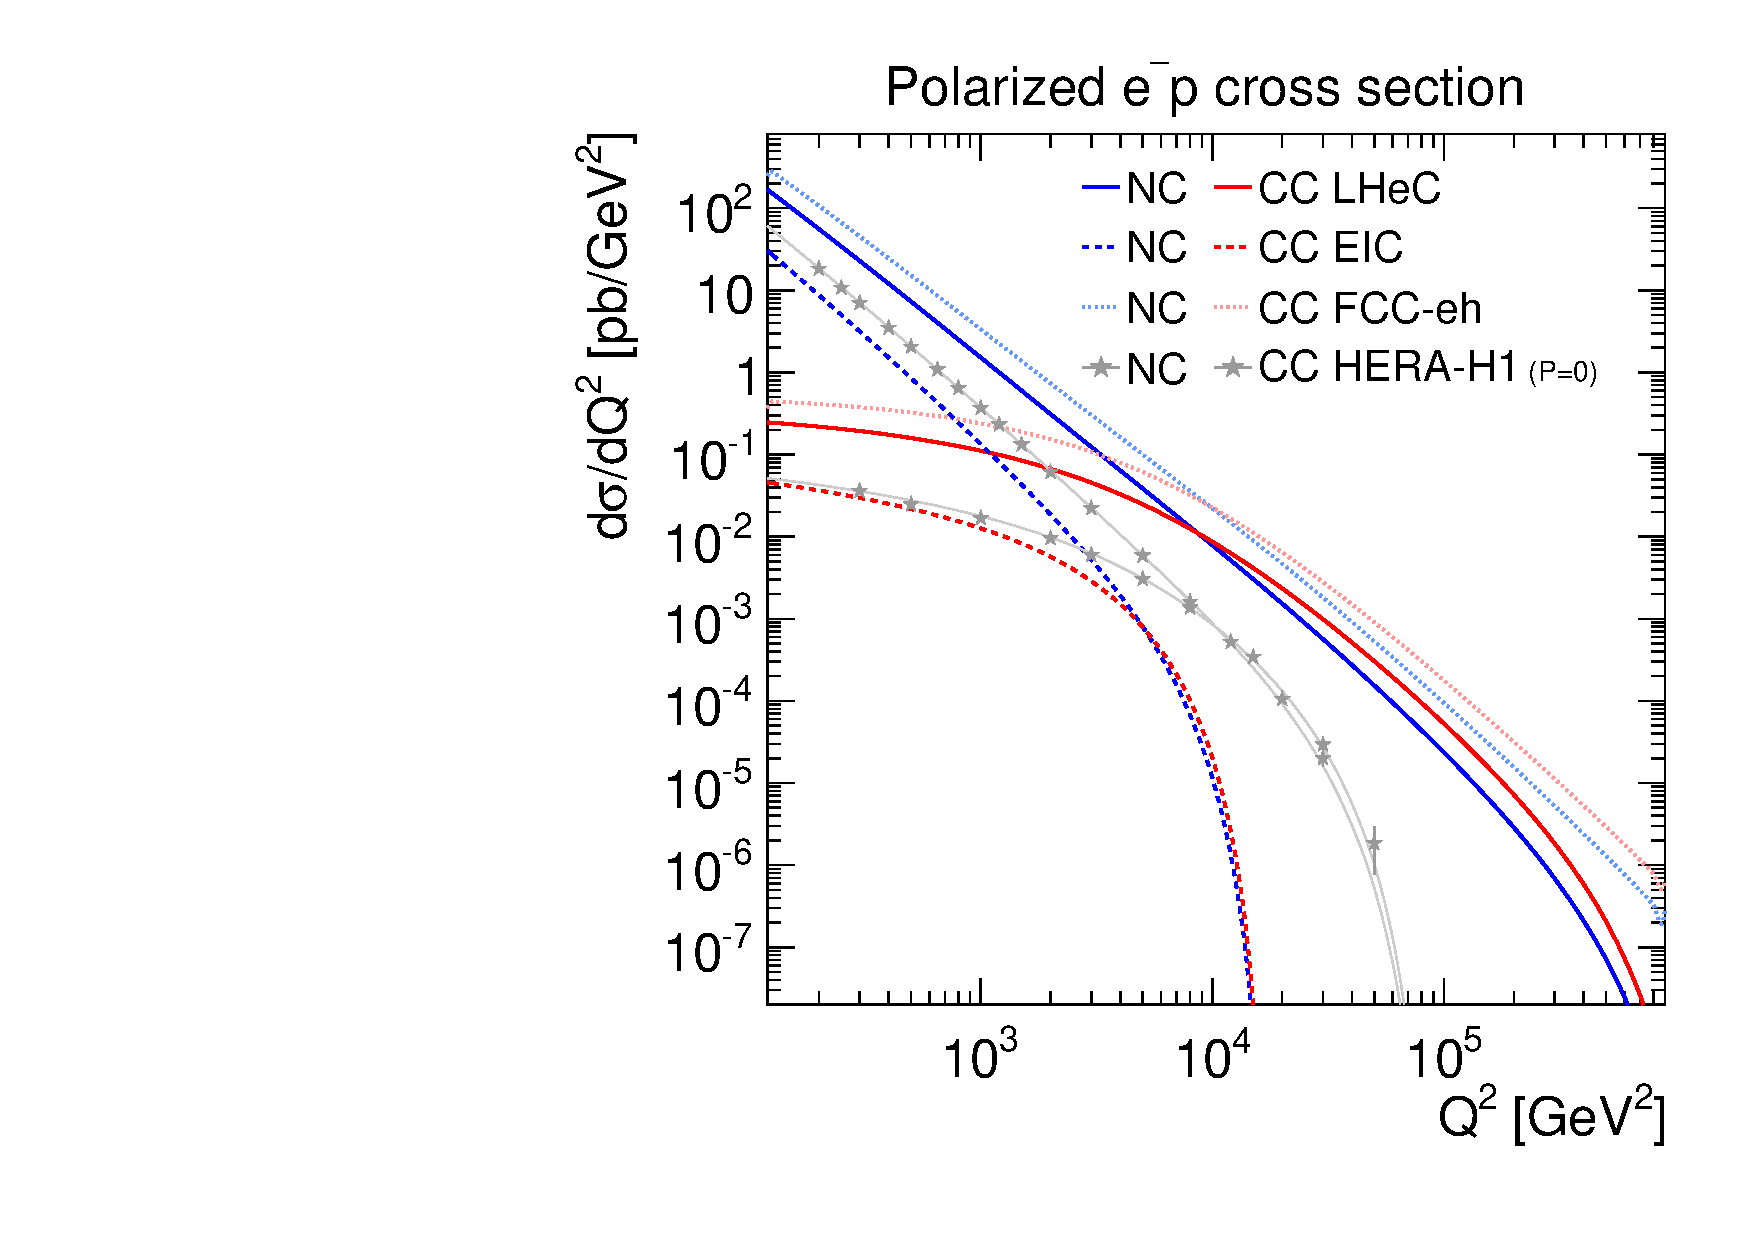
\includegraphics[width=0.52\textwidth]{plot_GraphsDsigmaDQ2_FCCEIC_opt}
  \caption{{Single differential inclusive DIS cross sections for
      $e^-p$ NC  and CC DIS at the
      EIC, HERA, LHeC and FCC-eh.
%      LHeC for two different electron beam energies
%      ($E_e=50\,\GeV$ and 60\,\GeV).
%      Cross sections for longitudinal
%      electron beam
%      polarisations of $P_e=-0.8$ and $+0.8$ are displayed.
%      For comparison also measurements at center-of-mass energies
%      of $\sqrt{s}=920$ by H1 at HERA for unpolarised ($P=0\,\%$)
%      electron beams are displayed.
  }}
  \label{fig:dSigmaFacilities}
\end{figure}

{\color{green}Two alternative versions of this plot are below}
\begin{figure}[h!b]
  \centering
  \includegraphics[width=0.38\textwidth]{plot_GraphsDsigmaDQ2_LHeC_opt}
  \hskip0.05\textwidth
  \includegraphics[width=0.38\textwidth]{plot_GraphsDsigmaDQ2_FCC_opt}
  \caption{
    Left: Inclusive NC and CC DIS cross sections as a function of \Qsq
    for two different polarisation states $P=\pm0.8$ and for two different electron
    beam energies, $E_e=50$ and $60\,\GeV$.
    For comparison, also the HERA measurements are displayed for $P=0$.
    Right: Inclusive NC and CC DIS cross sections as a function of
    \Qsq for different proton beam energies, $E_p=7$, 20 and
    50\,TeV. The latter two are possible at the future FCC.
    {\color{red} Appendix/additional figure?}
  }
  \label{fig:dSigmaopt}
\end{figure}

%-----------------------------------------------------------------------
%                            Summary
%-----------------------------------------------------------------------
\clearpage
\section{Summary and Conclusion}
\label{sect:Conclusion}
{\color{green} Text partially equivalent to the FCC-CDR}
%
Simulated neutral current and charged current inclusive DIS cross
sections at the LHeC are explored for a determination of the
fundamental parameters of electroweak theory and for precision tests
of the Standard Model formalism.
%
The high center-of-mass energy and the large integrated
luminosity at the LHeC will allow for the first time precision electroweak
measurement in DIS at high scales.
%


Highest precision is achieved for the measurement of the $W$-boson
mass with a prospected experimental uncertainty of up to
$\Delta\mW=5\,\MeV$, and an outstanding  
precision can also be achieved for the weak neutral current couplings of
light quarks to the $Z$ boson.
%
The space-like momentum transfer in DIS further allows for unique
scale dependent test of the electroweak theory, both, for neutral and
charged currents.
This includes for instance scale dependent measurements of the effective
weak mixing angle in the range of about $40<\sqrt{\Qsq}<700\,\GeV$
with a precision up to a few permille.

Further direct measurements, as for instance Higgs production,
top-quark production or single $W$ or $Z$
production cross sections, or vector-boson-scattering cross sections,
as well as heavy flavor cross sections in NC and CC DIS, will provide further
improvements for electroweak precision measurements.

The measurements will not be limited by the need for parton
distribution functions.
In many cases, the measurements are complementary to measurements in
$e^+e^-$ or hadron-hadron collisions.


In summary, the inclusive NC and CC DIS cross sections measured at
LHeC provide a unique opportunity to perform high-precision
determinations of fundamental electroweak parameters and test the
quantum  nature of electroweak processes with high precision.
Complementarity!

Unique measurements will be made for weak charged currents and
for the scale-dependence of electroweak interactions.

{\color{red}We studied in a traditional way NC and CC separately.
Many models predict changes to NC and CC simultaneously. A such, a
simultaneous determination of NC and CC observables is reasonable}



%-----------------------------------------------------------------------
%  Optional material, to be discussed...
%-----------------------------------------------------------------------
\clearpage
\section{Optional material}
\subsection{Electron couplings}
{\color{magenta} Todo: Discussion about \ve\ and \gae.}
\begin{figure}[htbp]
    \centering
    \includegraphics[width=0.40\textwidth]{plot_couplings_e}
  \caption{
    Weak-neutral-current vector and axial-vector couplings of the electron
    at 68\,\% confidence level~(C.L.) for
    simulated LHeC data with $E_e=60\,\GeV$.
    The LHeC expectations are compared with results from the combined
    analysis of LEP+SLD data~\cite{ALEPH:2005ab}, which are much more precise.
    {\color{red}We need to re-do this plot, but I don't know if it is
      at all reasonable to show it...}
  }
  \label{fig:couplings}
\end{figure}


% ------------------------------------------------------------------------ 
\clearpage
\subsection{Polarisation asymmetry in NC, and polarisation in CC}
Results from  more specific fits of
$\sin^2\theta_\text{W}^{\text{eff},\ell}(\mz^2)$.

\begin{table}[htb]
  \centering
  \small
  %\begin{tabular}{lr@{\hskip4pt}lccc}
  \begin{tabular}{lcccccc}
    \toprule
    Fit parameters &  Parameter & SM & \multicolumn{4}{c}{Expected uncertainties} \\
    \cmidrule(lr){4-7}
    &   of interest  &  value    & LHeC-50 & LHeC-60 & LHeC-50 & LHeC-60 \\
    &                &          &  \multicolumn{2}{c}{\footnotesize{($\delta_\text{uncor.}=0.50\,\%$)}} & \multicolumn{2}{c}{\footnotesize{($\delta_\text{uncor.}=0.25\,\%$)}} \\
    \midrule
    $\kappa^\prime_{\text{NC},f}$, PDFs
    & $\sin^2\theta_\text{W}^{\text{eff},\ell}(\mz^2)$ & 0.23154 & $0.00033$ & $0.00025$ & 0.00022 & $0.00015$ \\ % ok
    $\kappa^\prime_{\text{NC},f}$, $\rho^\prime_{\text{NC},f}$, PDFs
    & $\sin^2\theta_\text{W}^{\text{eff},\ell}(\mz^2)$ & 0.23154 & 0.00071  & 0.00036 &  0.00056 & 0.00023 \\ %ok
    $\kappa^\prime_{\text{NC},e}$, PDFs
    &  $\sin^2\theta_\text{W}^{\text{eff},e}(\mz^2)$   & 0.23154 & $0.00059$  & $0.00047$ & 0.00038 & $0.00028$ \\
    $\kappa^\prime_{\text{NC},e}$, $\kappa^\prime_{\text{NC},u}$, $\kappa^\prime_{\text{NC},d}$, PDFs
    &  $\sin^2\theta_\text{W}^{\text{eff},e}(\mz^2)$   & 0.23154 & 0.00111 & 0.00095 & 0.00069 & 0.00056\\ %ok
%    \midrule
    $\kappa^\prime_{\text{NC},f}$
    & $\sin^2\theta_\text{W}^{\text{eff},\ell}(\mz^2)$ & 0.23154 & 0.00028 & 0.00023 & 0.00017 & 0.00014 \\ % ok
    \bottomrule
    % kappa' fit with PDFs:
    %  0.00033 & 0.00025 & 0.00022 & 0.00015
    % kappa' fit without PDFs:
    %  0.00028 & 0.00023 & 0.00017 & 0.00014
    %    $\sin^2\theta_\text{W}^{\text{eff},\ell}$ (PDG)      & $0.23148$    & $\pm0.00013$    \\
    %    $\sin^2\theta_\text{W}^{\text{eff},\ell}$ (LEP+SLD)  & $0.23154$    & $\pm0.00016$    \\
    %    $\sin^2\theta_\text{W}^{\text{eff},\ell}$ (Tevatron) & $0.23148$    & $\pm0.00033$    \\
    %    $\sin^2\theta_\text{W}^{\text{eff},\ell}$ (LHC)      & $0.23131$    & $\pm0.00033$    \\
    %    $\sin^2\theta_\text{W}^{\text{eff},\ell}$ ($A_{fb}^{0,\ell}$ LEP)  & $0.23099$    & $\pm0.00053$    \\
%\hline
  \end{tabular}
  \caption{
    Determination of $\sin^2\theta_\text{W}^{\text{eff},\ell}(\mz^2)$
    with inclusive DIS data at the LHeC for different scenarios.
    Since the value of the effective weak mixing angle at the $Z$ pole
    cannot be determined directly in DIS, a fit of the
    $\kappa^\prime_{\text{NC},f}$ parameter is performed instead and
    its uncertainty is translated to
    $\sin^2\theta_\text{W}^{\text{eff},\ell}(\mz^2)$.
    Different assumptions on the fit parameters are studied, and
    results include uncertainties from the PDFs.
    Only the last line shows results where the PDF parameters are kept fixed.
    See text for more details.
    {\color{red}Not yet referenced and discussed in the text.}
  }
  \label{tab:sweff}
\end{table}



% ------------------------------------------------------------------------ 
\clearpage
\subsection{Best uncertainties for $\rho^\prime$ and $\kappa^\prime$
  parameters}
In a fit of a single anomalous form factor, we obtain following uncertainties. 
{\color{blue} Maximum sensitivity is obtained in 1-parameter fits, and prospects are collected in table:~\ref{tab:rhopwithcorrelations}.}
\begin{table}[bhtp]
  \footnotesize
  \centering
  \begin{tabular}{lcr@{$\,\pm\,$}lr@{$\,\pm\,$}l}
    \hline
    Fit parameters & Parameter & \multicolumn{2}{c}{LHeC}& \multicolumn{2}{c}{FCC}  \\
    \hline
    \rhopu+PDF & \rhopu &  1  &  0.009    & 1  & 0.004  \\
    \kappu+PDF & \kappu &  1  &  0.004    & 1  & 0.003  \\
    \rhopd+PDF & \rhopd &  1  &  0.014    & 1  & 0.006  \\
    \kappd+PDF & \kappd &  1  &  0.023    & 1  & 0.013  \\
    \rhope+PDF & \rhope &  1  &  0.006    & 1  & 0.003  \\
    \kappe+PDF & \kappe &  1  &  0.003    & 1  & 0.002  \\
    \hline
    \rhopq+PDF & \rhopq &  1  &  0.0059    & 1  & 0.0027  \\
    \kappq+PDF & \kappq &  1  &  0.0038    & 1  & 0.0024  \\
    \hline
    \rhopf+PDF & \rhopf &  1  &  0.0031    & 1  & 0.0015  \\ %0.00145641
    \kappf+PDF & \kappf &  1  &  0.0019    & 1  & 0.0011  \\
    \hline
    \\
    \multicolumn{3}{l}{Expectations for \rhopW{,f} (CC)} \\
    \hline
    % log.final.PAR19eq50.3p.PDF.2.txt
    \rhopW{,f}+PDF   & \rhopW{,f}                &  1  &   0.0043  & 1  & 0.0027 \\
    \rhopW{,eq}+PDF  & \rhopW{,eq}               &  1  &   0.0027  & 1  &  0.0011\\
    \rhopW{,e\bar{q}}+PDF  & \rhopW{,e\bar{q}}   &  1  &   0.0030  & 1  &  0.0012\\
    \hline
  \end{tabular}
  \caption{
    {\color{red} note: these numbers need to be updated, if we want to
    include such a table.}
    Results for $\rhop{}$, $\kapp{}$ and \rhopW{} parameters.
  }
  \label{tab:rhopwithcorrelations}
\end{table}




% ------------------------------------------------------------------------ 
\clearpage
\subsection{Polarisation asymmetry in NC, and polarisation in CC}
{\color{green}A potential additional plot could be about the
  polarisation asymmetry, but this maybe opens a long discussion...}
\begin{figure}[h!b]
\begin{center}
   \includegraphics[width=0.40\textwidth]{{figures/fcc_asymmetry}.pdf}
   \hskip1cm
   \includegraphics[width=0.40\textwidth]{{figures/fcc_CCtot}.pdf}
\end{center}
\caption{
  Left: Neutral-current polarisation asymmetry as a function of
  \Qsq\ integrated over $x$ for FCC-eh simulated data. The polarisation asymmetry
  is displayed for pure photon exchange, which is zero
  by definition, % due to the absence of parity violating terms.
  for calculations including only the interference terms $\gamma^*Z$,
  and for predictions including also purely weak effects, $ZZ$.
  The full circles illustrate simulated data points, which have
  uncertainties invisible at the chose scales.
  Right: Charged-current cross sections measured with different lepton
  polarisation states and for electron (red) and positron
  (blue) beams. The full circles illustrate FCC-eh simulated data,
  whereas the open circles show H1 measurements. The data are scaled
  by the the center-of-mass energies of the respective collider.
  The error bars are smaller than the markers.
}
\label{fig:crosssections}
\end{figure}


%-----------------------------------------------------------------------
%                          Acknowledgements
%-----------------------------------------------------------------------
\clearpage
\section*{Acknowledgements}
Acknowledgements: Z.~Zhang, A.~Sch\"oning, M.~Klein, S.~Schmitt



%-----------------------------------------------------------------------
%\input{fcc_draft}


%-----------------------------------------------------------------------
%   Results from LHeC inclusive DIS data
%-----------------------------------------------------------------------
\clearpage
\section{Tables}
\subsection{Determinations of single parameters}
\begin{table}[h]
  \footnotesize
  \centering
  \begin{tabular}{lcr@{$\,\pm\,$}lr@{$\,\pm\,$}l}
    \hline
    Fit parameters & Parameter & \multicolumn{2}{c}{LHeC}& \multicolumn{2}{c}{FCC}  \\
    \hline
    % log.fcc.6p.u.d.e.txt
    % EPRC.rhopu                =            1   +/-   0.00864794
    % EPRC.zkapu                =            1   +/-   0.00886882
    % EPRC.rhopd                =            1   +/-   0.028591
    % EPRC.zkapd                =            1   +/-   0.0438381
    % EPRC.rhope                =            1   +/-   0.0136914
    % EPRC.zkape                =            1   +/-   0.00510635
    \rhopd+\kappd+\rhopu+\kappu+\rhop{,e}+\kapp{,e}+PDF
    & \rhopu &  1  &  0.031    & 1  & 0.009 \\
    & \kappu &  1  &  0.013    & 1  & 0.009 \\
    & \rhopd &  1  &  0.062    & 1  & 0.029   \\
    & \kappd &  1  &  0.076    & 1  & 0.044  \\
    & \rhope &  1  &  0.036    & 1  & 0.014  \\
    & \kappe &  1  &  0.008    & 1  & 0.005 \\
    \hline
    % /nfs/dust/h1/group/britzger/alpos/Alpos/../log.fcc.4p.u.d.txt
    % EPRC.rhopu                =            1   +/-   0.00748481
    % EPRC.zkapu                =            1   +/-   0.00663437
    % EPRC.rhopd                =            1   +/-   0.0159018
    % EPRC.zkapd                =            1   +/-   0.0419873
    %lhec
    % EPRC.rhopu                =            1   +/-   0.0185425
    % EPRC.zkapu                =            1   +/-   0.0102184
    % EPRC.rhopd                =            1   +/-   0.0394555
    % EPRC.zkapd                =            1   +/-   0.0757502
    \rhopd+\kappd+\rhopu+\kappu+PDF
    & \rhopu &  1  &  0.019  & 1  & 0.007   \\
    & \kappu &  1  &  0.010  & 1  & 0.007   \\
    & \rhopd &  1  &  0.039  & 1  & 0.016   \\
    & \kappd &  1  &  0.076  & 1  & 0.042   \\
    \hline
    % /nfs/dust/h1/group/britzger/alpos/Alpos/../log.fcc.4p.e.q.txt
    %rhopq                     =            1   +/-   0.00827489
    %zkapq                     =            1   +/-   0.005199
    %EPRC.rhope                =            1   +/-   0.0100664
    %EPRC.zkape                =            1   +/-   0.00504328
    \rhop{,q}+\kapp{,q}+\rhop{,e}+\kapp{,e}+PDF
    & \rhop{,q} & 1 &  0.029  & 1 &  0.008  \\
    & \kapp{,q} & 1 &  0.007  & 1 &  0.005 \\
    & \rhop{,e} & 1 &  0.032  & 1 &  0.010 \\
    & \kapp{,e} & 1 &  0.008  & 1 &  0.005 \\
    \hline
    % /nfs/dust/h1/group/britzger/alpos/Alpos/../log.fcc.4p.e.q.txt
    %rhopq                     =            1   +/-   0.00827489
    %zkapq                     =            1   +/-   0.005199
    %EPRC.rhope                =            1   +/-   0.0100664
    %EPRC.zkape                =            1   +/-   0.00504328
    \rhop{,q}+\kapp{,q}+\rhop{,e}+\kapp{,e}+PDF
    & \rhop{,q} & 1 &  0.029  & 1 &  0.008  \\
    & \kapp{,q} & 1 &  0.007  & 1 &  0.005 \\
    & \rhop{,e} & 1 &  0.032  & 1 &  0.010 \\
    & \kapp{,e} & 1 &  0.008  & 1 &  0.005 \\
    \hline
    % /nfs/dust/h1/group/britzger/alpos/Alpos/
    \rhopu+\kappu+PDF
    & \rhopu &  1  &  0.011    & 1 & 0.005\\
    & \kappu &  1  &  0.005    & 1 & 0.003\\
    \hline
    % /nfs/dust/h1/group/britzger/alpos/Alpos/
    \rhopd+\kappd+PDF
    & \rhopd &  1  &  0.022    &  1  & 0.011 \\
    & \kappd &  1  &  0.038    &  1  & 0.021 \\
    \hline
    \rhop{,e}+\kapp{,e}+PDF
    & \rhope &  1  & 0.009      & 1  & 0.005 \\
    & \kappe &  1  & 0.005      & 1  & 0.003  \\
    \hline
    \rhop{,f}+\kapp{,f}+PDF
    & \rhope &  1  & 0.0042      & 1  & 0.0022 \\
    & \kappe &  1  & 0.0026      & 1  & 0.0016  \\
    \hline
    \\
    \multicolumn{3}{l}{Fits including \rhopW{,f} (CC)} \\
    \hline
    % log.final.PAR19eq50.3p.PDF.2.txt
    \rhop{,f}$+$\kapp{,f}$+$\rhopW{,f}+PDF
    & \rhop{f}   &  1  &  0.0045   & 1  & 0.0021 \\
    & \kapp{f}   &  1  &  0.0027   & 1  & 0.0015 \\
    & \rhopW{,f} &  1  &  0.0043   & 1  & 0.0027 \\
    % & $\rhop{W,f}=1.002\pm0.008$ & \\
    \hline
  \end{tabular}
  \caption{
    Results for $\rhop{}$, $\kapp{}$ and \rhopW{} parameters, and their
    correlation coefficients.
  }
  \label{tab:rhopwithcorrelations}
\end{table}


\begin{table}[h]
  \footnotesize
  \centering
  \begin{tabular}{lr@{$\,=\,$}c@{$\,\pm\,$}l|cccccc}
    \hline
    Fit parameters & \multicolumn{3}{c}{Result} & \multicolumn{6}{l}{Correlation} \\
    \hline
    % /nfs/dust/h1/group/britzger/alpos/Alpos/
    \rhopd+\kappd+\rhopu+\kappu+\rhop{,e}+\kapp{,e}+PDF
    & \rhopu &    &      & 1.00 \\
    & \kappu &    &      & 0.  & 1.00 \\
    & \rhopd &    &      &$    $& $   $ & 1.00 \\
    & \kappd &    &      &$    $& $   $ &  & 1.00 \\
    & \rhope &    &      &      &       &  &      &  1.00 \\
    & \kappe &    &      & 0.   &       &  &      &  & 1.00 \\
    \hline
    % /nfs/dust/h1/group/britzger/alpos/Alpos/
    \rhopd+\kappd+\rhopu+\kappu+PDF
    & \rhopu &    &      & 1.00 \\
    & \kappu &    &      & 0.  & 1.00 \\
    & \rhopd &    &      &$    $& $   $ & 1.00 \\
    & \kappd &    &      &$    $& $   $ &  & 1.00 \\
    \hline
    % /nfs/dust/h1/group/britzger/alpos/Alpos/
    \rhop{,q}+\kapp{,q}+\rhop{,e}+\kapp{,e}+PDF
    & \rhop{,e} &    &     & 1.00 \\
    & \kapp{,e} &    &     & 0.  & 1.00 \\
    & \rhop{,q} &    &     &     & 0.  & 1.00 \\
    & \kapp{,q} &    &     & 0.  & $0$ & 0.0  & 1.00 \\
    \hline
    % /nfs/dust/h1/group/britzger/alpos/Alpos/
    \rhopu+\kappu+PDF
    & \rhopu &    &      & 1.00 \\
    & \kappu &    &      & 0.  & 1.00 \\
    \hline
    % /nfs/dust/h1/group/britzger/alpos/Alpos/
    \rhopd+\kappd+PDF
    & \rhopd &    &      & 1.00 \\
    & \kappd &    &      &  & 1.00 \\
    \hline
    % /nfs/dust/h1/group/britzger/alpos/Alpos/
    \rhop{,e}+\kapp{,e}+PDF
    & \rhope &    &      &  1.00 \\
    & \kappe &    &      &  & 1.00 \\
    \hline
    \\
    \multicolumn{3}{l}{Fits including \rhopW{,f} (CC)} \\
    \hline
    % log.final.PAR19eq50.3p.PDF.2.txt
    \rhop{,f}$+$\kapp{,f}$+$\rhopW{,f}+PDF
    & \rhop{f}   &    &     & 1.00 & \\
    & \kapp{f}   &    &     & 0. & 1.00  \\
    & \rhopW{,f} &    &     & 0. & $0.$ & 1.00\\
    % & $\rhop{W,f}=1.002\pm0.008$ & \\
    \hline
  \end{tabular}
  \caption{
    Results for $\rhop{}$, $\kapp{}$ and \rhopW{} parameters, and their
    correlation coefficients.
  }
  \label{tab:rhopwithcorrelations}
\end{table}


% ------------------------------------------------------------------------
%
% ------------------------------------------------------------------------
\clearpage
\section*{Useless stuff}
%Reasonable examples are determinations of (all) the weak neutral current
%couplings, $g_A^{f}$ and $g_V^{f}$ with $f=(e,u,d,s,c,b,t)$,
%or more general, directly the $\rho_{\text{NC}, f}$ and
%$\kappa_{\text{NC}, f}$ parameters.
These can be done either in the scale-indpendent LO approximation, by
taking the scale-dependent loop corrections from theory, or their
effective values can be determined at different scales.
More commonly though, the effective weak mixing
angle $\sin\theta_{\text{W}}^{\text{eff},f}:=\kappa_{\text{NC}, q/e}\ \sw$
is tested at different scales, while also this quantity has an
important scheme dependent component (see Ref.~\ref{pdg18} for a
concise dicsussion).
Noteworthy, most of the precision measurements are performed in the
time-like domain, i.e.\ for $\mu^2>0$, whereas DIS is mediated by space-like
momentum transfer, $\Qsq=-q^2$, and thus $q^2<0$.
In DIS at the LHeC, in addition, a large kinematic range can be tested.

Complementary, the measurement of the weak boson masses yields an interesting testing
case of the theory, in particular the measurement of \mw.
This is because \mw\ can be considered as input parameter to the
formalism, or alternatively, if the precision measurement of \gf\ is
been taken as input~\cite{Tishchenko:2012ie}, then \mw becomes a
prediction and can be confronted with the measurement directly.
